\clearpage
\chapter{Sample RGA chromosomes}
\label{appendix:chromos}

\begin{figure}[htp]
\centerline{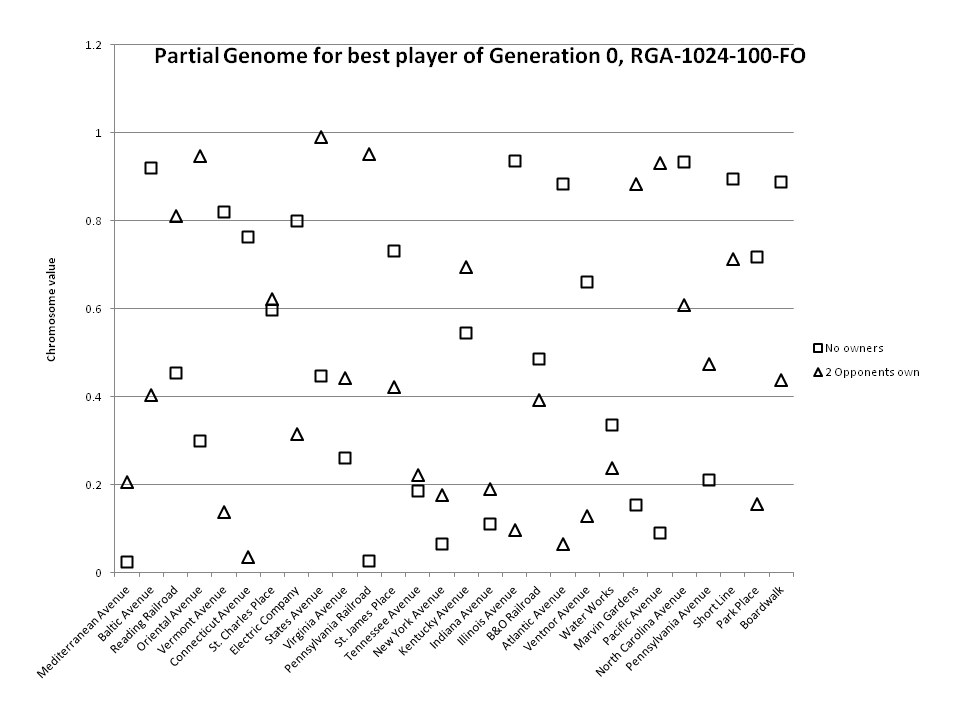
\includegraphics[width=0.75\columnwidth]{Figures/genome000.png}}
\caption[Illustration of Genome, Generation 0]{This chart shows part of the
genome of the fittest player in the first generation of the RGA-1024-100-FO
population. This chart compares the chromosome used when no player owns
any property in the group (represented by the square symbol) against the
chromosome used when two other players own a property in the group (the triangle
symbol).}
\label{app:figure-genome0}
\end{figure}

\begin{figure}[htp]
\centerline{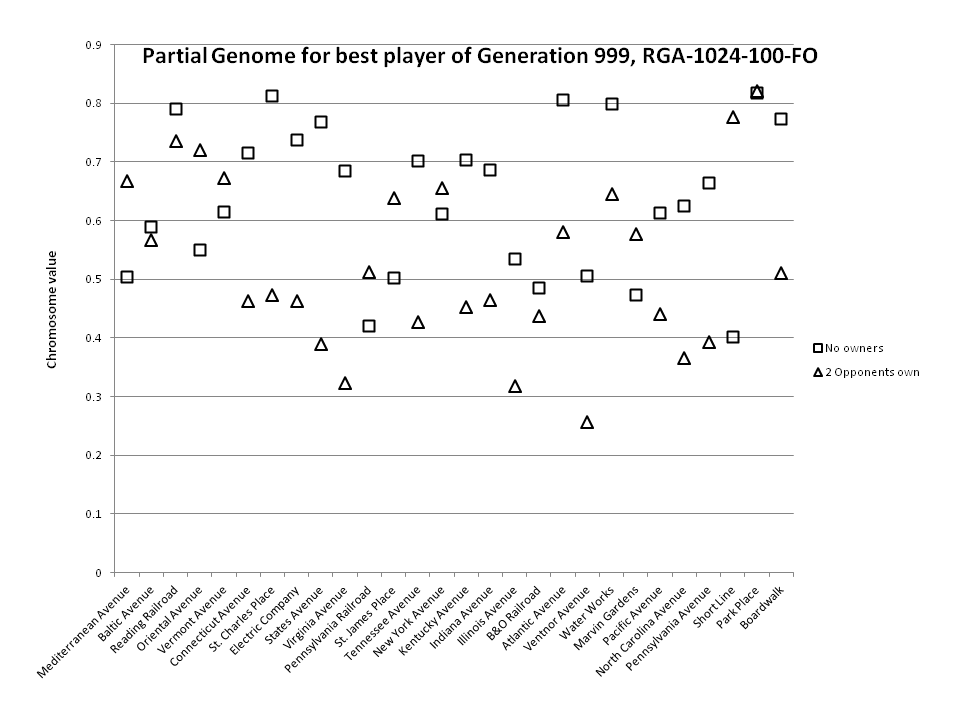
\includegraphics[width=0.75\columnwidth]{Figures/genome999.png}}
\caption[Illustration of Genome, Generation 999]{This chart shows part of the
genome of the fittest player in the last generation of the RGA-1024-100-FO
population. This chart compares the chromosome used when no player owns any
property in the group (the square symbol) against the chromosome used when two
other players own a property in the group (the triangle symbol). These two genes
show agreement with the heuristic strategy: the player is more likely to buy a
property when no one owns a property in the group, and relatively less likely to
buy a property when other players are blocking the group from being
monopolized.}
\label{app:figure-genome999}
\end{figure}

% Table generated by Excel2LaTeX from sheet 'genome0099 (2)'
\begin{table}[htbp]
  \centering
  \caption[Genome Comparison, Gen 0 vs Gen 999]{Comparison of Best Genomes from Generation 0 and Generation 999}
  \scalebox{0.75}{
    \begin{tabular}{lrrr|rrr}
    \toprule
           & \multicolumn{3}{c|}{Generation 0} & \multicolumn{3}{c}{Generation 999} \\
    \midrule
           & No Owner & 2 Opponents own & Diff   & No Owner & 2 Opponents own & Diff \\
    Mediterranean Avenue & 0.023  & 0.205  & -0.182 & 0.504  & 0.668  & -0.164 \\
    Baltic Avenue & 0.920  & 0.404  & 0.517  & 0.589  & 0.567  & 0.023 \\
    Reading Railroad & 0.454  & 0.810  & -0.356 & 0.790  & 0.736  & 0.054 \\
    Oriental Avenue & 0.300  & 0.947  & -0.648 & 0.550  & 0.721  & -0.171 \\
    Vermont Avenue & 0.821  & 0.138  & 0.683  & 0.614  & 0.673  & -0.059 \\
    Connecticut Avenue & 0.762  & 0.036  & 0.726  & 0.715  & 0.463  & 0.252 \\
    St. Charles Place & 0.598  & 0.622  & -0.024 & 0.812  & 0.473  & 0.339 \\
    Electric Company & 0.799  & 0.314  & 0.484  & 0.737  & 0.463  & 0.274 \\
    States Avenue & 0.448  & 0.991  & -0.543 & 0.768  & 0.389  & 0.379 \\
    Virginia Avenue & 0.260  & 0.442  & -0.182 & 0.685  & 0.323  & 0.362 \\
    Pennsylvania Railroad & 0.027  & 0.952  & -0.925 & 0.421  & 0.512  & -0.091 \\
    St. James Place & 0.730  & 0.423  & 0.308  & 0.502  & 0.639  & -0.137 \\
    Tennessee Avenue & 0.186  & 0.223  & -0.036 & 0.702  & 0.427  & 0.275 \\
    New York Avenue & 0.064  & 0.175  & -0.111 & 0.612  & 0.656  & -0.043 \\
    Kentucky Avenue & 0.544  & 0.694  & -0.150 & 0.704  & 0.452  & 0.252 \\
    Indiana Avenue & 0.110  & 0.189  & -0.080 & 0.686  & 0.465  & 0.221 \\
    Illinois Avenue & 0.936  & 0.096  & 0.840  & 0.536  & 0.319  & 0.217 \\
    B\&O Railroad & 0.487  & 0.391  & 0.095  & 0.485  & 0.437  & 0.048 \\
    Atlantic Avenue & 0.884  & 0.064  & 0.820  & 0.806  & 0.581  & 0.225 \\
    Ventnor Avenue & 0.661  & 0.128  & 0.532  & 0.506  & 0.257  & 0.250 \\
    Water Works & 0.335  & 0.237  & 0.098  & 0.800  & 0.645  & 0.154 \\
    Marvin Gardens & 0.154  & 0.883  & -0.730 & 0.472  & 0.577  & -0.104 \\
    Pacific Avenue & 0.091  & 0.931  & -0.840 & 0.614  & 0.440  & 0.173 \\
    North Carolina Avenue & 0.934  & 0.609  & 0.325  & 0.625  & 0.365  & 0.260 \\
    Pennsylvania Avenue & 0.210  & 0.474  & -0.265 & 0.663  & 0.392  & 0.271 \\
    Short Line & 0.895  & 0.713  & 0.182  & 0.402  & 0.778  & -0.376 \\
    Park Place & 0.718  & 0.155  & 0.563  & 0.818  & 0.822  & -0.004 \\
    Boardwalk & 0.887  & 0.439  & 0.448  & 0.774  & 0.511  & 0.263 \\
    \bottomrule
    \end{tabular}}
  \label{apptab:chromo_compare}%
\end{table}%

